%-------------------------------------------------------------------
% Document class and package definitions
%-------------------------------------------------------------------
\documentclass[12pt,a4paper,openany,final,oneside]{cseethesis}

%Included for Gather Purpose only:
%input "thesisreferences.bib"

%%%%%% MATH SYMBOLS DEFINED HERE %%%%%%%%%%%
\makenomenclature

\nomenclature{\(a\)}{Speed of light in a vacuum}
\nomenclature{\(b\)}{Planck constant}
\nomenclature{\(c\)}{Speed of light in a vacuum}
\nomenclature{\(d\)}{Planck constant}
\nomenclature{\(e\)}{Speed of light in a vacuum}
\nomenclature{\(f\)}{Planck constant}
\nomenclature{\(g\)}{Speed of light in a vacuum}
\nomenclature{\(h\)}{Planck constant}
\nomenclature{\(i\)}{Speed of light in a vacuum. This is a very long description of a mathematical symbol used throughout the document}
\nomenclature{\(j\)}{Planck constant}
\nomenclature{\(k\)}{Speed of light in a vacuum}
\nomenclature{\(l\)}{Planck constant}
\nomenclature{\(m\)}{Speed of light in a vacuum}
\nomenclature{\(n\)}{Planck constant}
\nomenclature{\(o\)}{Speed of light in a vacuum}
\nomenclature{\(p\)}{Planck constant}
\nomenclature{\(q\)}{Speed of light in a vacuum}
\nomenclature{\(r\)}{Planck constant}
\nomenclature{\(s\)}{Speed of light in a vacuum}
\nomenclature{\(u\)}{Planck constant}
\nomenclature{\(v\)}{Speed of light in a vacuum. So that's why this list is very cool and stuff plase subscribe to my channel}
\nomenclature{\(w\)}{Planck constant}
\nomenclature{\(x\)}{Speed of light in a vacuum}
\nomenclature{\(y\)}{Planck constant}
\nomenclature{\(z\)}{Speed of light in a vacuum}
\nomenclature{\(å\)}{Planck constant}
\nomenclature{\(ä\)}{Speed of light in a vacuum}
\nomenclature{\(ö\)}{Planck constant. Wow so many long symbol desciptions and yet the list stays aligned. Very cool wouldn't you say}

%%%%%%%%%%%%%%%%%%%%%%%%%%%%%%%%%%%%%%%%%%%%

%-------------------------------------------------------------------
% Glim's additions
%-------------------------------------------------------------------

%Packages

\usepackage{todonotes}
\setuptodonotes{
  size=\small,          % font size inside note
  color=orange!80,        % background color
  linecolor=red,       % connector color
}

%Fic todo note overflow
\setlength{\marginparwidth}{2cm} % tweak 2.2–3.0cm as needed



%This is just to change the color of the note arrow
\usepackage{etoolbox}
\makeatletter
% Right margin line
\patchcmd{\@todonotes@drawLineToRightMargin}
  {\tikzstyle{both}=[line width=3pt, draw, opacity=0.15]}
  {\tikzstyle{both}=[line width=3pt, draw=\@todonotes@currentlinecolor, opacity=0.6]}
  {}{}
% Left margin line
\patchcmd{\@todonotes@drawLineToLeftMargin}
  {\tikzstyle{both}=[line width=3pt, draw, opacity=0.15]}
  {\tikzstyle{both}=[line width=3pt, draw=\@todonotes@currentlinecolor, opacity=0.6]}
  {}{}
\makeatother



\usepackage[most]{tcolorbox}



%Custom commands
\newtcolorbox{draftnote}{
  colback=cyan!30!white,     % light cyan background
  %colbacklower=cyan!30!white,% darker cyan lower half
  colframe=black,            % black border
  coltitle=white,            % title text color
  fontupper = \small \bfseries,
  fonttitle=\bfseries,       % bold title
  title=Draft Note,       % box title
  width=\textwidth,          % span full text width
  boxrule=1pt,               % border thickness
  arc=5pt,                   % rounded corners
  center
}

\newcommand{\note}[1]{%
  \begin{draftnote}#1\end{draftnote}%
}



\newcommand{\now}{
\todo[inline, color = red!70!white]{\color{white}
\begin{center}  
$\downarrow$ \textbf{CURRENT WORKING LOCATION} $\downarrow$ 
\end{center}}
}

% --- DEFINE COLORS ---
\definecolor{x}{HTML}{1395BA}   % teal (F_x)
\definecolor{y}{HTML}{F5A623}   % amber (F_y)
\definecolor{tq}{HTML}{7B61FF}  % violet (tau)
\definecolor{edge}{HTML}{222222}  % dark gray edges
\definecolor{healthy}{HTML}{2ECC71}   % green (healthy thruster)
\definecolor{failed}{HTML}{E74C3C}    % red (failed thruster)

\newcommand{\x}[1]{\textcolor{x}{#1}}      % teal (F_x)
\newcommand{\y}[1]{\textcolor{y}{#1}}      % amber (F_y)
\newcommand{\tq}[1]{\textcolor{tq}{#1}}    % violet (tau)
\newcommand{\edge}[1]{\textcolor{edge}{#1}} % charcoal (neutral)
\newcommand{\ok}[1]{\textcolor{healthy}{#1}}   % green (healthy)
\newcommand{\fail}[1]{\textcolor{failed}{#1}}  % red (failed)

\newcommand{\thr}[5]{% corner, dx, dy, state(on/off), \TL
        \pgfmathsetmacro{\dx}{#2}
        \pgfmathsetmacro{\dy}{#3}
        \path (#1) coordinate (C);
        \path let \p1 = (C) in coordinate (T) at (\x1 - #5*\dx, \y1 - \TL*\dy);
        \ifthenelse{\equal{#4}{on}}{%
            \draw[thrOn] (C) -- (T);
        }{%
            \draw[thrOff] (C) -- (T);
        }%
    }


\newcommand{\body}{
 % --- parameters ---
    \def\a{0.20}   % half side of slider
    \def\TL{0.1}   % arrow length

    % --- styles ---
    \tikzset{
        slider/.style={fill=black!8, draw=edge, thick},
        thrOn/.style={-Stealth, line width=1.2pt, draw= healthy},
        thrOff/.style={-Stealth, line width=1.2pt, draw=failed, dashed}
    }

    % --- slider body ---
    \path (-\a,-\a) coordinate (BL)
          (\a,-\a)  coordinate (BR)
          (\a,\a)   coordinate (TR)
          (-\a,\a)  coordinate (TL);
    \filldraw[slider] (TL)--(TR)--(BR)--(BL)--cycle;
}

\begin{document}

\defaultbibliography{thesisreferences}     %% Change this only.
\defaultbibliographystyle{plain}        %% Could be changed if you like 
                                           %% references typeset differently.
%-------------------------------------------------------------------
% Define title, author, etc.
%-------------------------------------------------------------------
\def\thesistitle{Fault Tolerant Control}

\def\theauthor{Glim\ Lindaregård}
\def\theaddress{Dept.\ of Computer Science, Electrical and Space Engineering\\
Lule{\aa} University of Technology\\ Lule{\aa}, Sweden}

\def\supervisors{Avijit Banerjee (Luleå University of Technology)}
\def\supervisorstring{Supervisors:} % Edit here if you have only one supervisor
\def\dedication{Ingenjör? Inget gör}

% Read abstract and preface from separate files.
% Make sure these exist. See example files.
\def\theabstract{\input{abstract.tex}}
\def\thepreface{Acknowledgements here\\[2.5cm]
Luleå, August 2025\\
Glim \ Lindaregård}


% Change here if you want to remove the logo printed on the first page

%\def\thelogo{\includegraphics[width=2.5cm]{bg_wall.jpg}} % old EU logo
\def\thelogo{} % no logo

% The definitions above could be put directly in the function call below,
% but is here defined explicitly, for the purpose of clarity.

\startpreamble
  {\thesistitle}
  {\theauthor}
  {\theaddress}
  {\supervisors}
  {\dedication}
  {\theabstract}
  {\thepreface}
  {\thelogo}

%%%%%%%%%%%%%%%%%%%%%%%%%%%%%%%%%%%%%%%%%%%%%%%%%%%%%%%%%%%%%%%%%%%%
%% Begin Part I
%%%%%%%%%%%%%%%%%%%%%%%%%%%%%%%%%%%%%%%%%%%%%%%%%%%%%%%%%%%%%%%%%%%%
%\makepartpage{Part I}


%% Initialize part containing the thesis introduction chapters
\startchapters
\begin{bibunit}
%------------------------ Start chapter 1 --------------------------
% The \makechapter command takes three arguments
%  1) An abbreviated version of the chapter name,
%     to be used as page header
%  2) String to be added to the table of contents
%  3) The chapter name, possibly split in to lines,
%     as in Chapter 2 below.
%
%  The different arguments can have different line breaks.
%
% The actual contents of the chapter is included by removing the
% comment from the \input line below. Make sure the file
% chapter1.tex exists.
%-------------------------------------------------------------------

\makechapter{Introduction}{Introduction}{Introduction\label{introduction}}
\input{Chapters/1 introduction/introduction}

\makechapter{Background}{Background}{Background\label{background}}
{
\let\clearpage\relax
\let\newpage\relax
\let\pagebreak\relax

\begin{tcolorbox}[  colback=cyan!30!white,     % light cyan background
  %colbacklower=cyan!30!white,% darker cyan lower half
  colframe=black,            % black border
  coltitle=white,            % title text color
  fontupper = \small \bfseries,
  fonttitle=\bfseries,       % bold title
  title=Draft Note,       % box title
  width=\textwidth,          % span full text width
  boxrule=1pt,               % border thickness
  arc=5pt,                   % rounded corners
  center,
  width = 0.9\textwidth]
  
  Something like: Here we will introduce the different components of a \gls{FTCS}, how they work together, historical and current methods, and finish be explaining the literature gap for this thesis.

\end{tcolorbox}

\begin{tcolorbox}
    hi
\end{tcolorbox}
    

\section{Problem Context and Fault Models}
Here we will intruduce the differnet types of relevant faults and assumptions.
\todo[inline]{I think we could do some cool graphics here, describing the faults.}
\begin{itemize}
    \item \textbf{Actuator faults:} Loss-of-effectiveness (LoE), stuck-on/off, bias, saturation.

    \item \textbf{Sensor faults:} bias, drift, dropout, complete outage.

    \item \textbf{Contraints:} actuator limits (torque, thrust, rate)

    \item \textbf{Inertia and velocity sensing assumption:} Most spacecraft FTC studies consider the inertia tensor uncertain, since on-orbit conditions (propellant slosh, deployable structures) can shift the mass distribution. In contrast, the present air-bearing testbed has a rigid body with fixed, measurable inertia, so inertia is treated as known.

Another spacecraft-specific theme is velocity sensing. Many CubeSats exclude gyros to save cost and power, relying only on attitude sensors (e.g., star trackers, magnetometers). This motivates “velocity-free FTC” designs, where angular rates are reconstructed with observers. The testbed provides direct rate measurements, but the velocity-free paradigm remains an important thread in spacecraft FTC literature.
\end{itemize}




\section{Basics of Fault-Tolerant Control}
% This section will introduce the main ideas and methods used in \ac{FTC}. Moving forward in this section, classification follows the layout presented in \cite{Zhang2008BibliographicalSystems}. Zhang categorizes \ac{FTC} methods up until 2008. Methods developed after 2008 will have their own reference. 


A closed-loop control system capable of accommodating actuator faults while retaining its performance capability is said to be a \textit{Fault-Tolerant Control System}. Such a system is critical in systems such as \ac{S/C} and nuclear facilities, among others. 

A \ac{FTCS} can be put in two main categories, \textbf{passive} and \textbf{active}. A \ac{PFTCS} uses a robust controller designed to handle a handful of pre-programmed failures. This method has a number of advantages; no \ac{FDD} is necessary since the controller never expects to know what has gone wrong, it simply observes a new sensor input and uses its robust control scheme to compensate. No controller reconfiguration including parameter recalculation and reconfiguration lag. This method is, however, limited in its ability to handle severe faults. In contrast, \ac{AFTCS}'s uses sensors to identify faults, reconfigure the control system in such a way as to use the remaining actuators as efficiently as possible. 
\todo[inline]{Analogy? really?}
Imagine you are driving home from work, and suddenly you hit a nail and puncture your tire. Lucky for you, you just installed new run-flat tires (tires that continue to work even when punctured, albeit with a reduced efficiency), allowing you to continue your drive at a slower speed. This is \ac{PFTCS}, the run-flat tire handled the fault and allowed the car to continue operation at a reduced pace. A \ac{AFTCS} could have used a pressure sensor in the tire to realize when the tire was punctured, and automatically deploy a tire repair kit. This way, you can continue driving the car with no problems. \todo{might be silly analogy..}

\subsection{FTC Structure}

The figure below \todo{Ill make my own figure} depicts the general structure for a \ac{AFTCS}. As we will see, different control systems vary greatly in block choices and structure. This figure should thus not be seen as an absolute but rather serve as a first principles visual aid. \todo{holy wording...} Some of the blocks in the figure (Actuators, Sensors, and System) \todo[fancyline]{fix with new figure} are not explicitly explain and will be explained in detail in later chapters. Some additional blocks are not in the figure, these blocks are not fundamental and are only explained in the text. \todo[fancyline]{real?}

\begin{figure}[H]
    \centering
    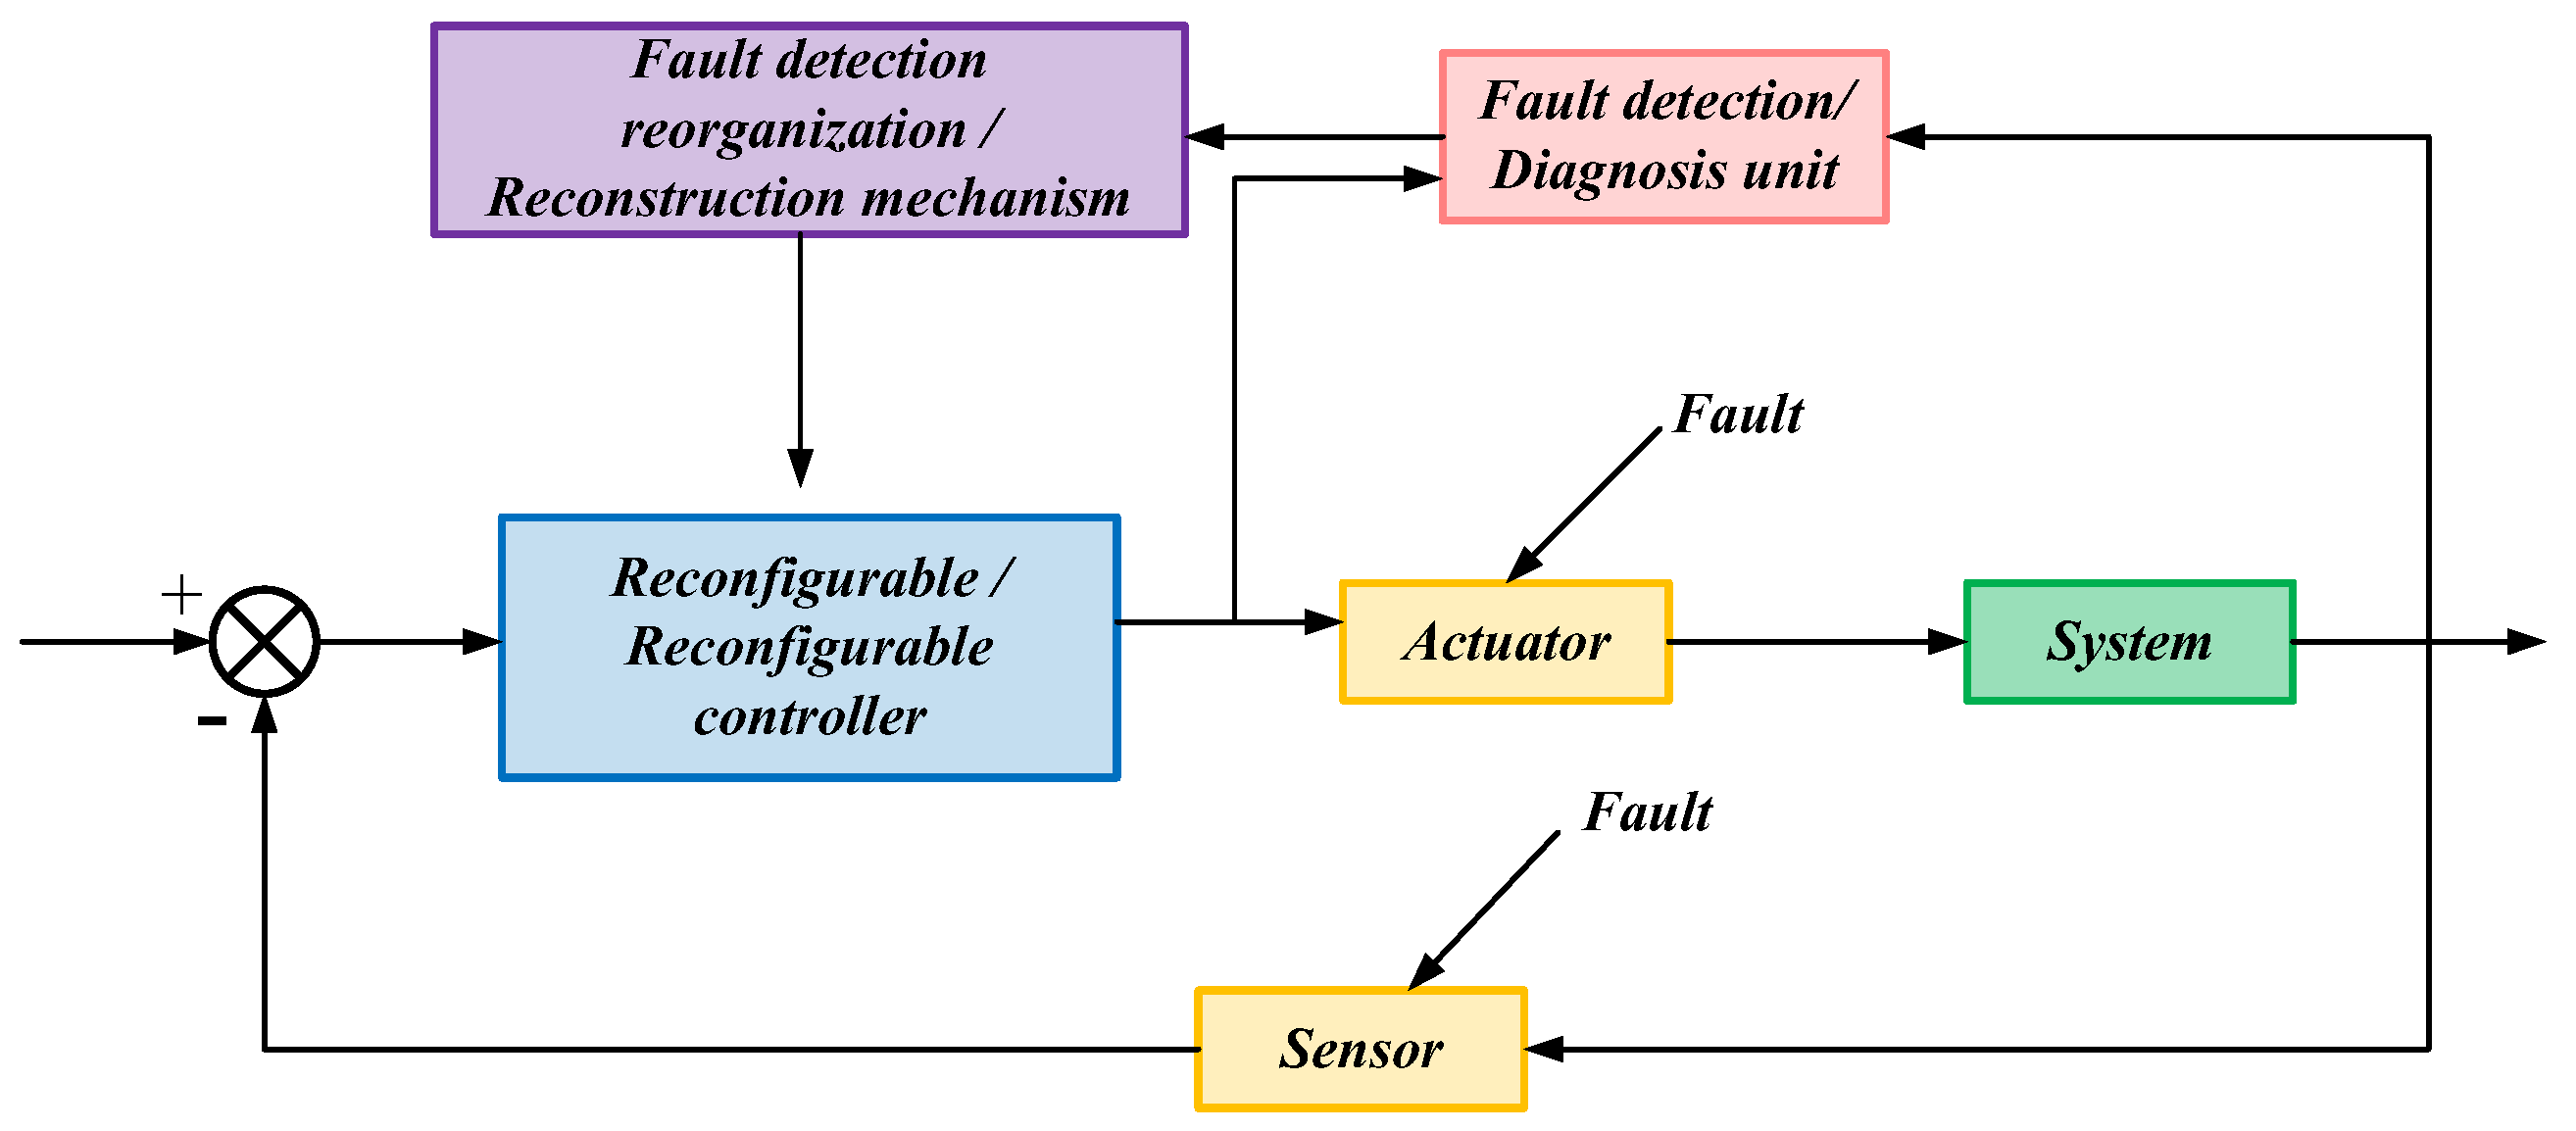
\includegraphics[width=0.5\linewidth]{images/basic_AFTCS.png}
    \caption{General structure of AFTCS}
    \label{fig:enter-label}
\end{figure}


\begin{itemize}

    \item \textbf{\ac{FDD} unit:} The \ac{FDD} could take inputs from various parts of the system depending on the design, but in general it takes signals outputted by the controller and compares them with the real-world effect.  This comparison can then lead to a conclusion on what has happened and report this to the \ac{RCU}.


    \item \textbf{\ac{RCU}:} This block listens to the \ac{FDD} unit for faults. Once a fault is detected, the \ac{RCU} reconfigures the controller to account for the new dynamics. The way the reconfiguration is performed can vary drastically and is part of what classifies the system as we will learn later.
    
    \item \textbf{Reconfigurable controller:} The reconfigurable controller acts as a normal controller during normal operations. Once the \ac{RCU} sends a reconfiguration request the controller will change in some way. As mentioned earlier, the way the controller change changer with design. 

    
    \item \textbf{Additional optional blocks (not in the figure \todo[fancyline]{or are they :) hmmmm}): } 
    \begin{itemize}
        \item \emph{\ac{CA}:} Usefull in over actuated systems where control effort can be redistributed over the functioning actuators. 

        \item \emph{Decision Layer:} Relatively new technique utilizing something like Behavior trees or \ac{NN} to orchestrate a multitude of strategies within a single system, switching to the most optimal strategy for the current situation.

        \item \emph{Reference/Command Governors:} filters that modify commands so they stay within actuator limits. In spacecraft FTC, they prevent saturation or instability after faults by slowing or reshaping reference signals without changing the controller.
    \end{itemize}

    
\end{itemize}

% \begin{itemize}
%     \item Definition and Taxonomy of FTC, importance in spacecraft systems.\\
%     A close-loop control system capable of accommodating actuator faults while retaining performance capability is said to be a \textit{Fault Tolerant Control System :) }
%     \item Active vs. Passive FTC:
%         \begin{itemize}
%             \item Active FTC relies on Fault Detection and Diagnosis (FDD) with controller reconfiguration.
%             \item Passive FTC uses fixed controllers designed to tolerate a range of faults.
%         \end{itemize}
%     \item System components: controller, FDD scheme, reconfiguration mechanism, command/reference governor.
%     \item Key references: Zhang \& Jiang (2008), Jiang \& Yu (2012), Yin et al. (2016).
% \end{itemize}

\section{Controller Law Families}
Controllers come in a multitude of flavors. Some are designed to withstand gradual faults, while others are designed to stabilize a \gls{S/C} after a total thruster failure. Worth mentioning before this section is that no controller, whether it be \gls{SMC}, \gls{MPC}, or a PID, is inherently active/passive, nor are they robust, adaptive, or intelligent. The terms come from the system structure around the controller.

\subsection{Robust Control}

\gls{RC} refers to control methods designed to maintain stability and acceptable performance in the presence of bounded uncertainties and disturbances \cite{Zhang2008BibliographicalSystems,Jiang2012Fault-tolerantApproaches}. Unlike adaptive schemes, robust controllers are fixed once implemented; they rely on conservative design margins rather than online adjustment \cite{Jiang2012Fault-tolerantApproaches}.

Classical examples include $H_\infty$ control, which minimizes the worst-case disturbance amplification, as well as $\mu$-synthesis and reliable control formulations \cite{Yin2016ASystem}. These approaches are especially attractive when actuator faults or parameter variations can be bounded in advance, allowing the controller to absorb the effects without reconfiguration. For spacecraft, robust designs based on $H_\infty$ have been proposed for attitude stabilization under disturbances and partial actuator degradations, providing stability guarantees without requiring explicit fault diagnosis \cite{Yin2016ASystem}.

The main limitation of robust control is that performance is guaranteed only within the predefined uncertainty set. Larger or unexpected faults may exceed the controller’s robustness margins, leading to degraded performance or instability. For this reason, robust controllers are often used as passive FTC baselines, or combined with reconfiguration mechanisms in an active FTC framework to expand their fault coverage \cite{Zhang2008BibliographicalSystems,Jiang2012Fault-tolerantApproaches}.

\subsection{Sliding Mode Control (SMC)}
  \gls{SMC} is a nonlinear control approach that forces the system trajectory onto a predefined “sliding surface,” where the reduced-order dynamics are stable and robust to matched uncertainties \cite{Yin2016ASystem,Mirshams2014PassiveThrusters}. Its strength lies in handling abrupt actuator faults and external disturbances without requiring an exact model of the spacecraft dynamics. Variants such as terminal SMC and fixed-time SMC guarantee convergence to the desired state within bounded time \cite{Cao2013FaultMode}, while velocity-free SMC formulations eliminate the need for direct angular-rate measurements by employing state observers \cite{Guo2019Velocity-freeSaturation}
.

In spacecraft applications, SMC has been demonstrated as particularly effective for thruster-actuated platforms. For example, Mirshams et al. \cite{Mirshams2014PassiveThrusters} showed that an SMC-based design could maintain attitude stability after discrete thruster failures, leveraging the inherent robustness of the sliding surface dynamics. These properties make SMC attractive for \gls{FTC} scenarios where actuators fail in an on/off manner, a common fault mode in spacecraft propulsion systems.

However, SMC also carries limitations. The well-known chattering effect—caused by high-frequency switching—can excite unmodeled dynamics and degrade performance \cite{Yang2023AdaptiveFaults}. Moreover, SMC does not naturally account for input constraints such as actuator saturation, which are ubiquitous in spacecraft. To address these shortcomings, recent research explores hybrid approaches that combine SMC with optimization-based allocation or predictive control, enabling constraint handling while preserving robustness \cite{Khodaverdian2023Fault-tolerantSpacecraft}
.


\subsection{Adaptive Control}
\gls{AC} methods adjust controller parameters online to compensate for changing dynamics or actuator effectiveness. In the context of \gls{FTC}, they are particularly suited for gradual or parametric faults, such as partial loss of actuator authority or slow variations in inertia \cite{Jiang2012Fault-tolerantApproaches,Yin2016ASystem}. Rather than relying on fixed gains, an adaptive law continuously estimates system changes and updates the controller in real time.

Common spacecraft implementations include \\
\gls{MRAC}, which enforces tracking of a predefined reference model despite actuator failures \cite{Ma2014ActuatorFeedback}, and adaptive backstepping, which provides stability guarantees while compensating for parametric uncertainties \cite{Bustan2014AdaptiveControl}. Adaptive extensions of other families, such as adaptive SMC \cite{Yang2023AdaptiveFaults} and adaptive control allocation \cite{Tohidi2016FaultSpace}, have also been proposed to broaden fault tolerance while preserving robustness.

The strength of adaptive control lies in its ability to recover performance smoothly without explicit controller switching or redesign \cite{Jiang2012Fault-tolerantApproaches}. However, this benefit comes at the cost of slower response to abrupt, discrete faults, since adaptation requires time to estimate and converge to new parameters \cite{Zhang2008BibliographicalSystems}. Furthermore, the stability and effectiveness of adaptive FTC depend strongly on the accuracy of the fault estimation and the tuning of the adaptation law. Poor estimation quality can lead to oscillations or even instability, which has motivated hybrid designs that combine adaptive controllers with robust supervisory layers \cite{Zhang2008BibliographicalSystems,Jiang2012Fault-tolerantApproaches}.

\subsection{Intelligent, Fuzzy, and Learning-Based Control} 
\gls{FTC} methods increasingly explore intelligent and data-driven approaches that complement or replace model-based designs with heuristic or learning-based adaptation. \gls{FLC}s use linguistic rules (“if actuator efficiency decreases, then increase control effort”) to compensate for faults without requiring precise mathematical models. This makes them effective for gradual or ambiguous degradations, where exact fault dynamics are uncertain \cite{Zhang2008BibliographicalSystems,Yin2016ASystem}. Adaptive fuzzy controllers have been applied to spacecraft attitude control, demonstrating resilience to actuator faults by updating rule weights online\cite{Zou2011AdaptiveSpacecraft}
.

Beyond fuzzy logic, \gls{NN}s and \gls{RL} extend the paradigm by learning nonlinear mappings or control policies from data. \gls{NN}s can approximate unmodeled actuator or sensor fault effects, while \gls{RL} agents can directly learn fault-tolerant policies through trial-and-error optimization. For spacecraft, these approaches are promising for complex and poorly modeled faults such as partial thruster degradations or sensor bias. Recent work has demonstrated RL-based fault-tolerant attitude control, where an agent learns to stabilize a satellite despite actuator faults \cite{Rafiee2024ActiveFaults}.

While intelligent controllers offer flexibility, they remain less flight-proven than robust or adaptive methods. Stability guarantees are weaker, and their certification for space missions is challenging. As a result, fuzzy, neural, and RL-based approaches are most commonly found in simulations or laboratory testbeds rather than operational spacecraft \cite{Zhang2008BibliographicalSystems,Yin2016ASystem}. Ongoing research therefore focuses on hybrid strategies that combine learning-based adaptation with robust supervisory control, aiming to merge the flexibility of intelligent methods with the assurance required for safety-critical spacecraft operations.


\section{Reconfiguration Mechanisms}
Reconfiguration mechanisms are the means by which a control system adapts after a fault has been detected. Their role is to modify how control actions are applied so that stability and performance can be maintained under degraded conditions. While the previous section focused on control strategies, this section considers the mechanisms that put those strategies into practice.

\subsection{Controller Switching:} 
Controller switching is one of the earliest forms of reconfiguration. When a fault is detected, the active controller is replaced by another designed for the new condition. This method is simple and effective if the fault scenarios are known in advance, but it requires a library of pre-designed controllers, which grows quickly with system complexity.

Its success depends on fast and reliable fault detection, as poor or delayed switching can harm performance. Modern work often frames controller switching within hybrid control theory to improve robustness.

\subsection{Parameter Update and Compensation}
Another form of reconfiguration is to adjust the controller itself by updating parameters or adding compensation terms. Instead of switching controllers or redistributing commands, the existing control law is modified to account for the fault.

This approach can maintain continuity in control and avoid the abrupt changes that come with switching. Its effectiveness, however, depends on accurate fault estimation and timely adaptation. If the update is slow or incorrect, performance can degrade significantly.

\subsection{Control Allocation} 
Control allocation addresses how overall control commands are distributed among the available actuators. After a fault, the mechanism adjusts this distribution so that the remaining actuators can still generate the required forces and moments as closely as possible.

This strategy is particularly relevant in systems with actuator redundancy, such as spacecraft. Its strength lies in exploiting the extra degrees of freedom to maintain controllability despite failures. The specific algorithms for allocation—ranging from linear algebra methods to optimization—are discussed in detail in the following chapter.
\todo[inline]{This might not belong here}


\section{Thruster Allocation Methods}
Methods for allocating controll outputs to functioning actuators. 

\subsection{Pseudoinverse}
One of the most common allocation techniques is based on the Moore–Penrose pseudoinverse, which provides the least-squares actuator command vector that reproduces a desired torque or force. For spacecraft, this has been widely applied as a baseline allocation scheme because of its simplicity and computational efficiency \cite{Johansen2013ControlSurvey,Shen2015Inertia-freeAllocation}. A weighted pseudoinverse can down-weight faulty actuators or prioritize certain axes, while the null-space freedom of the solution allows secondary objectives such as fuel balancing or plume avoidance to be incorporated without disturbing the primary torque \cite{Durham1993ConstrainedAllocation}. The main limitation is that pseudoinverse allocation does not enforce actuator constraints (saturation, minimum impulse bit), which may lead to infeasible commands in practice.

\now






\section{Decision Layer and Governors}
Here we will introduce the decision making framework that orchestrate different FTC strategies.


\begin{itemize}
    \item \textbf{Behaviour trees:} modular, hierarchical logic to pick between FTC strategies.

    \item \textbf{Mode logic and switching rules:} older but common in aerospace

    \item  \textbf{Reference/Command Governors:} upervisory filters that keep commands within safety bounds.
\end{itemize}

FTC isen't just about the controller, its about the logic that chooses what to apply when.

\section{Performance Wrappers}
Here we intrduce some terms and ideas to be added on top. 
\todo[inline]{This might be too much...}
\begin{itemize}
    \item \textbf{Prescribed performance control (PPC):} guarantees on overshoot, steady-state error, settling time.

    \item \textbf{Finite-time and fixed-time stabilization:} guarantees bounded recovery time. 

    \item \textbf{Anti-saturation designs:} explicit handling of actuator limits.
\end{itemize}


These are newer methods that are now standard. 

\section{State of the Art and Trends (2008 to 2016 to 2022)}
Historical FTC overview
\todo[inline]{This might be too much. Think we already talk about this in the earlier text}
\note{The world of \ac{FTC} methods is a big game of mix and match of all the concepts and methods presented in this chapter.  Zhang \& Jiang (2008) \cite{Zhang2008BibliographicalSystems} gives a overview. }

Purpose: Give a historical and critical overview of how FTC evolved.

Content:

Zhang (2008): the original taxonomy, active vs passive, restructuring vs augmentation, FDI coupling.

Yin (2016): spacecraft focus, rise of velocity-free and allocation-centric designs.

Zhou (2022): critical assessment introducing controller-basis vs performance-basis perspectives; calls for event-triggered, model-free, less-redundancy-dependent FTC.

Why: This section shows the trajectory of the field and positions your work as part of this evolution




\section{Literature Gap and Thesis Positioning}
\todo[inline]{Need to figure out what this is... }

\subsection{Gaps and Directions for Comparative Study}
\begin{itemize}
    \item Fragmentation: control, allocation, and supervisory approaches often studied in isolation.
    \item Validation gap: limited hardware or high-fidelity simulation validation in spacecraft contexts.
    \item Research opportunity: systematic comparative study of candidate methods on a 2-D air-bearing testbed using ROS/Gazebo.
\end{itemize}


\todo[inline]{ROS/Gazebo here or in method?}
\section{ROS}
\include{Chapters/2_background/sections/ROS}

\section{Gazebo}
\include{Chapters/2_background/sections/gazebo}




}


\makechapter{Implementation of Direct Allocation Method}{Implementation of Direct Allocation Method}{Implementation of Direct Allocation Method\label{Implementation}}
 {
 \let\clearpage\relax
 \let\newpage\relax
 \let\pagebreak\relax

 %\section{Rendezvous and Proximity Operations}
 %\include{Chapters/Chapter 2/Sections/rpo conops}

 }


\makechapter{Method}{Method}{Method\label{method}}
{
\let\clearpage\relax
\let\newpage\relax
\let\pagebreak\relax

\section{Workspace}
\include{Chapters/4_method/Sections/workspace}

\section{AMS Construction}
A system like the slider is described as a redundant system. This means that there are more actuators than theoretically necessary to produce any desired moment. For such a system, a method must be devised to allocate control authority to specific actuators in order to deliver the desired moment. One such method involves storing all possible actuator combinations locally on board the system. It turns out that storing the actuator combinations as a geometric hypercube with each vertex representing one set of actuators, simplifies the search for optimal actuation,  which will become evident in later chapters. 

This chapter details the process of transforming the set of possible actuator combinations into the corresponding set of attainable system moments, known as the \gls{AMS}




Define A explicitly from thruster positions and orientation angles (referring to earlier figure).

Explain how A transforms thruster forces  u into body moments 

Since the \gls{AMS} fully depends on the position, orientation, nd number of actuators of the system, it is a good idea to define these in a concise way. This is done by creating a matrix where each column represents an actuator. Each entry, i, of the actuator column defines the actuator's ability to produce a moment along the $i^{\text{th}}$ spatial direction. 


%For the slider, take thruster one (pos: top right (r,r), orientation: $\beta_1 = \frac{3±pi}{2}$). This thruster will produce a unit force in $-\y{y}$ equal to $\cos{\beta_1}$ together with a negative moment equal to $r(\cos{\beta_1} - \sin{\beta_1})$

\begin{tikzpicture}[scale=8, >=Stealth]

    \body

    % --- top-left corner (thrusters off) ---
    \thr{TL}{-1}{0}{off}{\TL}
    \thr{TL}{0}{1}{off}{\TL}

    % --- top-right corner (thrusters off) ---
    \thr{TR}{1}{0}{on}{\TL}
    \thr{TR}{0}{1}{off}{\TL}

    % --- bottom-left corner (only downward thruster on) ---
    \thr{BL}{-1}{0}{off}{\TL}
    \thr{BL}{0}{-1}{off}{\TL}

    % --- bottom-right corner (only downward thruster on) ---
    \thr{BR}{1}{0}{off}{\TL}
    \thr{BR}{0}{-1}{off}{\TL}

    % --- coordinate frame ---
    \coordinate (origin) at (0.55, 0);
    \draw[->, thick] (origin) -- ++(0.15, 0) node[right] {$x$};
    \draw[->, thick] (origin) -- ++(0, 0.15) node[above] {$y$};
    \fill (origin) circle (0.01);

    
    
    

\end{tikzpicture}


\begin{equation}
    \boldsymbol{A} =
    \begin{bmatrix}
        \cos\beta_1 & \cdots & \cos\beta_8 \\[4pt]
        \sin\beta_1 & \cdots & \sin\beta_8 \\[4pt]
        (r^y_1 \cos\beta_1 - r^x_1 \sin\beta_1) & \cdots & (r^y_8 \cos\beta_8 - r^x_8 \sin\beta_8)
    \end{bmatrix}
\end{equation}





\[
    \boldsymbol{\Omega} = \{ \boldsymbol{u} \mid u_{i,min} \le u_i \le u_{i,max}, \boldsymbol{u} \in \mathbb{R}^m \} \subset \mathbb{R}^m \
\]
where in the case of the slider with 8 thrusters,
\[
    \boldsymbol{u} = \begin{bmatrix}  T_1 & T_2 & T_3 & T_4 & T_5 & T_6 & T_7& T_8 \end{bmatrix}^T
    \quad , \quad u_{i,min} \le T_i \le u_{i,max}
\]

The boundary of $\boldsymbol{\Omega}$ denoted $\partial(\boldsymbol{\Omega)}$ contains the controls that map to the 


\begin{figure}[h!]
\centering
\textbf{Down-scaled slider (8 thrusters; only the two bottom thrusters ON)}\\[0.5em]

\begin{minipage}[t]{0.45\linewidth}
\centering
\begin{tikzpicture}[scale=8, >=Stealth]

    \body
    
        % --- Letter ---
    \node at (0,0) {\Large \textbf{B}};
    
    % --- top-left corner (thrusters off) ---
    \thr{TL}{-1}{0}{off}{\TL}
    \thr{TL}{0}{1}{off}{\TL}

    % --- top-right corner (thrusters off) ---
    \thr{TR}{1}{0}{off}{\TL}
    \thr{TR}{0}{1}{off}{\TL}

    % --- bottom-left corner (only downward thruster on) ---
    \thr{BL}{-1}{0}{off}{\TL}
    \thr{BL}{0}{-1}{on}{\TL}

    % --- bottom-right corner (only downward thruster on) ---
    \thr{BR}{1}{0}{off}{\TL}
    \thr{BR}{0}{-1}{on}{\TL}

\end{tikzpicture}
\end{minipage}
\begin{minipage}[t]{0.45\linewidth}
\centering
\begin{tikzpicture}[scale=8, >=Stealth]

    \body

    % --- Letter ---
    \node at (0,0) {\Large \textbf{B}};


    % --- top-left corner (thrusters off) ---
    \thr{TL}{-1}{0}{on}{\TL}
    \thr{TL}{0}{1}{off}{\TL}

    % --- top-right corner (thrusters off) ---
    \thr{TR}{1}{0}{on}{\TL}
    \thr{TR}{0}{1}{off}{\TL}

    % --- bottom-left corner (only downward thruster on) ---
    \thr{BL}{-1}{0}{off}{\TL}
    \thr{BL}{0}{-1}{off}{\TL}

    % --- bottom-right corner (only downward thruster on) ---
    \thr{BR}{1}{0}{off}{\TL}
    \thr{BR}{0}{-1}{off}{\TL}

    % % --- coordinate frame ---
    % \coordinate (origin) at (0.55, 0);
    % \draw[->, thick] (origin) -- ++(0.15, 0) node[right] {$x$};
    % \draw[->, thick] (origin) -- ++(0, 0.15) node[above] {$y$};
    % \fill (origin) circle (0.01);

\end{tikzpicture}
\end{minipage}

\vspace{25pt}

\begin{minipage}{0.45\linewidth}
\centering
\begin{tikzpicture}[scale=8, >=Stealth]

    \body

    % --- Letter ---
    \node at (0,0) {\Large \textbf{C}};

    % --- top-left corner (thrusters off) ---
    \thr{TL}{-1}{0}{off}{\TL}
    \thr{TL}{0}{1}{on}{\TL}

    % --- top-right corner (thrusters off) ---
    \thr{TR}{1}{0}{on}{\TL}
    \thr{TR}{0}{1}{off}{\TL}

    % --- bottom-left corner (only downward thruster on) ---
    \thr{BL}{-1}{0}{on}{\TL}
    \thr{BL}{0}{-1}{off}{\TL}

    % --- bottom-right corner (only downward thruster on) ---
    \thr{BR}{1}{0}{off}{\TL}
    \thr{BR}{0}{-1}{on}{\TL}

\end{tikzpicture}
\end{minipage}
\begin{minipage}{0.45\linewidth}
\centering
\begin{tikzpicture}[scale=8, >=Stealth]

   \body

    % --- Letter ---
    \node at (0,0) {\Large \textbf{D}};


    % --- top-left corner (thrusters off) ---
    \thr{TL}{-1}{0}{off}{\TL}
    \thr{TL}{0}{1}{on}{\TL}

    % --- top-right corner (thrusters off) ---
    \thr{TR}{1}{0}{off}{\TL}
    \thr{TR}{0}{1}{off}{\TL}

    % --- bottom-left corner (only downward thruster on) ---
    \thr{BL}{-1}{0}{off}{\TL}
    \thr{BL}{0}{-1}{off}{\TL}

    % --- bottom-right corner (only downward thruster on) ---
    \thr{BR}{1}{0}{off}{\TL}
    \thr{BR}{0}{-1}{on}{\TL}

    % % --- coordinate frame ---
    % \coordinate (origin) at (0.55, 0);
    % \draw[->, thick] (origin) -- ++(0.15, 0) node[right] {$x$};
    % \draw[->, thick] (origin) -- ++(0, 0.15) node[above] {$y$};
    % \fill (origin) circle (0.01);

\end{tikzpicture}
\end{minipage}



\caption{Eight thrusters (two per corner). Green arrows indicate active thrusters (on); red dashed arrows indicate inactive thrusters (off). The two bottom thrusters are active, producing upward thrust and a net lift.}
\label{fig:simple_slider_onoff}
\end{figure}






\begin{equation}
    \boldsymbol{\psi_d}^{n\times 1} = \boldsymbol{Au} = \begin{bmatrix} \color{x}f_x & \color{y}f_y &\color{tq} \tau\end{bmatrix}^T
\end{equation}

Where $\boldsymbol{u}^{m\times 1}$ is the control vector:


The set of all possible control inputs produced by the m thrusters span a convex hull in $\mathbb{R}^m$ control space: 




The control space is then transformed to the \gls{AMS} under the A map:

\[
    \boldsymbol{\Phi} = \{\boldsymbol{\psi} \mid \boldsymbol{\psi} = \boldsymbol{Au}, \boldsymbol{u} \in \boldsymbol{\Omega}\} \subset \mathbb{R}^n
\]

\todo[inline]{I dont know how detailed to describe the AMS construction method and what to reference to the original paper.}


% --- Plot simple slider --- 
\begin{figure}
    \centering
    \textbf{Down-scaled slider}\\[0.5em]
    \begin{tikzpicture}[scale=5, >=Stealth]
        \def\a{0.2}
    
        % --- main coordinates ---
        \coordinate (v0) at (0,0);
        \coordinate (v1) at (2*\a,0);
        \coordinate (v2) at (0,2*\a);
        \coordinate (v3) at (-2*\a,-2*\a);
    
        \coordinate (s1) at (\a, \a);
        \coordinate (s2) at (-\a, \a);
        \coordinate (s3) at (-\a, -\a);
        \coordinate (s4) at (\a, -\a);
    
        % --- transparent gray square ---
        \filldraw[fill=gray, fill opacity=0.2, draw=black, thick]
            (s1)--(s2)--(s3)--(s4)--cycle;
    
        % --- red vectors ---
        \draw[red, thick, -Stealth] (v0) -- (v1) node[pos=1,right,black] {u1};
        \draw[red, thick, -Stealth] (v0) -- (v2) node[pos=1,above,black] {u3};
        \draw[red, thick, -Stealth] (v0) -- (v3) node[pos=1,below left,black] {u2};

    
        % --- coordinate system to the right ---
        \coordinate (origin) at (0.6, 0); % move it wherever looks good
        \draw[->, black, thick] (origin) -- ++(0.15, 0) node[right] {$x$};
        \draw[->, black, thick] (origin) -- ++(0, 0.15) node[above] {$y$};
        \fill[black] (origin) circle (0.01); % small dot at the origin
    \end{tikzpicture}

    \caption{Red arrows represent the three thrusters, one in \x{\texttt{+x}}, one in \y{\texttt{+y}} and one in (\x{\texttt{-x}},\y{\texttt{-y}}). These thrusters only produce thrust in \x{\texttt{x}} and \y{\texttt{y}}, no moment or rotation.}
    \label{fig:simpleSlider}
\end{figure}

% --- Plot 3D CS and 2D AMS ---
\begin{figure}
    \centering
    \textbf{3D Control Space to 2D AMS Visualization}\\[0.5em]
    \tdplotsetmaincoords{75}{5}
    \begin{tikzpicture}[tdplot_main_coords, scale = 3,>=Stealth]

        % --- 2D hull points (z=0 plane) ---
        \coordinate (p0) at (0,0,0);
        \coordinate (p1) at (0,1,0);
        \coordinate (p2) at (1,1,0);
        \coordinate (p3) at (-1,0,0);
        \coordinate (p4) at (1,0,0);
        \coordinate (p5) at (0,-1,0);
        \coordinate (p6) at (-1,-1,0);
        
    
        % --- Hull polygon ---
        \filldraw[fill = cyan, fill opacity = 0.5, draw=black, thick]
            (p6) -- (p5) -- (p4) -- (p2) -- (p1) -- (p3) -- cycle;
    
        % --- Optionally mark vertices ---
        \foreach \p in {p1,p2,p3,p4,p5,p6}
            \fill[red] (\p) circle (0.04);

        % --- Vertices ---
        \coordinate (v1) at (0,0,0);
        \coordinate (v2) at (1,0,0);
        \coordinate (v3) at (1,1,0);
        \coordinate (v4) at (0,1,0);
        \coordinate (v5) at (0,0,1);
        \coordinate (v6) at (1,0,1);
        \coordinate (v7) at (1,1,1);
        \coordinate (v8) at (0,1,1);

       % --- Red arrows ---
       \foreach \v/\p in {
           v8/p3,
           v6/p2,
           v5/p1,
           v4/p6,
           v3/p5}
        {
        \draw[red,thick,-Stealth] (\v) -- (\p);
        }

        \draw[red, thick,-Stealth] (v7) -- (p0) node[black, pos = 0.98, anchor = north east] {$\mathbb{O}$};


        % --- Faces ---
        % bottom
        \filldraw[fill = cyan!99!black, draw = black, fill opacity = 0.2, thick] (v1)--(v2)--(v3)--(v4)--cycle;
        % front
        \filldraw[fill = cyan!99!black, draw = black, fill opacity = 0.2, thick] (v2)--(v6)--(v7)--(v3)--cycle;
        % right
        \filldraw[fill = cyan!99!black, draw = black, fill opacity = 0.2, thick] (v1)--(v5)--(v6)--(v2)--cycle;
        % left
        \filldraw[fill = cyan!99!black, draw = black, fill opacity = 0.2, thick] (v4)--(v8)--(v5)--(v1)--cycle;
        % back
        \filldraw[fill = cyan!99!black, draw = black, fill opacity = 0.2, thick] (v3)--(v7)--(v8)--(v4)--cycle;
        % top
        \filldraw[fill = cyan!99!black, draw = black, fill opacity = 0.2, thick] (v5)--(v6)--(v7)--(v8)--cycle;

        % --- Coordinate system aligned with cube (top-right corner plane) ---
        \coordinate (originCS) at (1.3, 1.1, 0);   % place it near top-right corner of cube
        
        % axis arrows: x→ right, y→ up in 2D plane, z→ upward (3D)
        \draw[->, black, thick] (originCS) -- ++(0.4, 0, 0) node[anchor=west] {$x$};
        \draw[->, black, thick] (originCS) -- ++(0, -0.8, 0) node[anchor=south east] {$y$};
        \draw[->, black, thick] (originCS) -- ++(0, 0, 0.4) node[anchor=south] {$z$};
        \fill[black] (originCS) circle (0.015);

    \end{tikzpicture}
    
    \caption{Control space (3D) to AMS (2D) transformation under $A = \begin{bmatrix}
        1 & -1 & 0 \\ 0 & -1 & 1
    \end{bmatrix}$. Red arrows represent vertex mappings from control space to AMS. ex: $[0\ 1\ 1]$ in control space maps to $[-1\ 0]$ in the AMS. This is saying that if thruster 2 and 3 is on we should move in -x, which is constantan with figure}
    \label{fig:simpleTransform}
    
\end{figure} 

\section{AMS Search}
\include{Chapters/4_method/Sections/AMS Search}


}

\makechapter{Results}{Results}{Results\label{results}}
% {
% \let\clearpage\relax
% \let\newpage\relax
% \let\pagebreak\relax

% \section{Evaluation of DT Simulation}
% \include{Chapters/Chapter 4/Sections/dt results}

% \section{Evaluation of HIL Testing}
% \include{Chapters/Chapter 4/Sections/hil results}

% \section{Evaluation of End-to-End Testing}
% \include{Chapters/Chapter 4/Sections/end end results}

% }


\makechapter{Analysis, Discussion, and Conclusions}{Analysis, Discussion, and Conclusions}{Analysis, Discussion, and Conclusions\label{analysis}}
% {
% \let\clearpage\relax
% \let\newpage\relax
% \let\pagebreak\relax

% % \section{Analysis}
% % % {
% \let\clearpage\relax
% \let\newpage\relax
% \let\pagebreak\relax

% % \section{Analysis}
% % % {
% \let\clearpage\relax
% \let\newpage\relax
% \let\pagebreak\relax

% % \section{Analysis}
% % \include{Chapters/Chapter 5/Sections/analysis}

% % \section{Discussion}
% % \include{Chapters/Chapter 5/Sections/discussion}

% % \section{Conclusions}
% % \include{Chapters/Chapter 5/Sections/conclusions}

% }

% % \section{Discussion}
% % \include{Chapters/Chapter 5/Sections/discussion}

% % \section{Conclusions}
% % \include{Chapters/Chapter 5/Sections/conclusions}

% }

% % \section{Discussion}
% % \include{Chapters/Chapter 5/Sections/discussion}

% % \section{Conclusions}
% % \include{Chapters/Chapter 5/Sections/conclusions}

% }

\makechapter{Continued Work, Research, and Recommendations}{Continued Work, Research, and Recommendations}{Continued Work, Research, and Recommendations\label{cont}}
% {
% \let\clearpage\relax
% \let\newpage\relax
% \let\pagebreak\relax

% % \section{Continued Work}
% % \include{Chapters/Chapter 6/Sections/contd work}

% % \section{Research}
% % \include{Chapters/Chapter 6/Sections/research}

% % \section{Recommendations}
% % \include{Chapters/Chapter 6/Sections/recom}

% }

\makebib
\end{bibunit}

\makeappendices

\end{document}
